\documentclass[11pt,a4paper]{article}
\usepackage[utf8]{inputenc}
\usepackage[margin=1in]{geometry}
\usepackage{graphicx}
\usepackage{amsmath}
\usepackage{listings}
\usepackage{float}
\usepackage{subcaption}
\usepackage{xcolor}
\usepackage{booktabs}

% Configure code listings
\lstset{
    language=Python,
    basicstyle=\ttfamily\footnotesize,
    keywordstyle=\color{blue},
    commentstyle=\color{green!60!black},
    stringstyle=\color{red},
    breaklines=true,
    frame=single,
    numbers=left,
    numberstyle=\tiny\color{gray}
}

\title{Intelligent Agents in Snake Game: \newline A Comparative Implementation Report}
\author{Python Journey - ML Snake Agents}
\date{\today}

\begin{document}

\maketitle

\begin{abstract}
This report presents and compares five intelligent agent architectures for the classic Snake game: Simple Reflex Agent, Goal-Based Agent, Utility-Based Agent, Model-Based Agent, and Q-Learning Agent. Each agent is described with its code implementation and illustrated with gameplay and score screenshots, demonstrating the progression from reactive to learning-based artificial intelligence.
\end{abstract}

\section{Introduction}
Intelligent agents are autonomous entities that perceive their environment and take actions to achieve specific objectives. In the Snake game, agents must collect food while avoiding collisions. This report demonstrates five agent types, each with increasing sophistication, culminating in a reinforcement learning agent that learns optimal strategies through experience.

% ===================== SIMPLE REFLEX AGENT =====================
\section{Simple Reflex Agent}
\subsection{Description}
The Simple Reflex Agent reacts to the current position of the apple, moving toward it if safe. It does not plan ahead or learn from experience.

\subsection{Code}
\begin{lstlisting}[caption=Simple Reflex Agent]
def simple_agent(game):
    head_x, head_y = game.snake.x[0], game.snake.y[0]
    apple_x, apple_y = game.apple.x, game.apple.y

    if apple_x < head_x:
        next_x, next_y = game._get_potential_head("left")
        if not game._is_potential_move_colliding(next_x, next_y):
            game.snake.move_left()
            return
    if apple_x > head_x:
        next_x, next_y = game._get_potential_head("right")
        if not game._is_potential_move_colliding(next_x, next_y):
            game.snake.move_right()
            return
    if apple_y > head_y:
        next_x, next_y = game._get_potential_head("down")
        if not game._is_potential_move_colliding(next_x, next_y):
            game.snake.move_down()
            return
    if apple_y < head_y:
        next_x, next_y = game._get_potential_head("up")
        if not game._is_potential_move_colliding(next_x, next_y):
            game.snake.move_up()
            return
# No fallback strategy
\end{lstlisting}

\subsection{Screenshots}
\begin{figure}[H]
    \centering
    \begin{subfigure}{0.45\textwidth}
        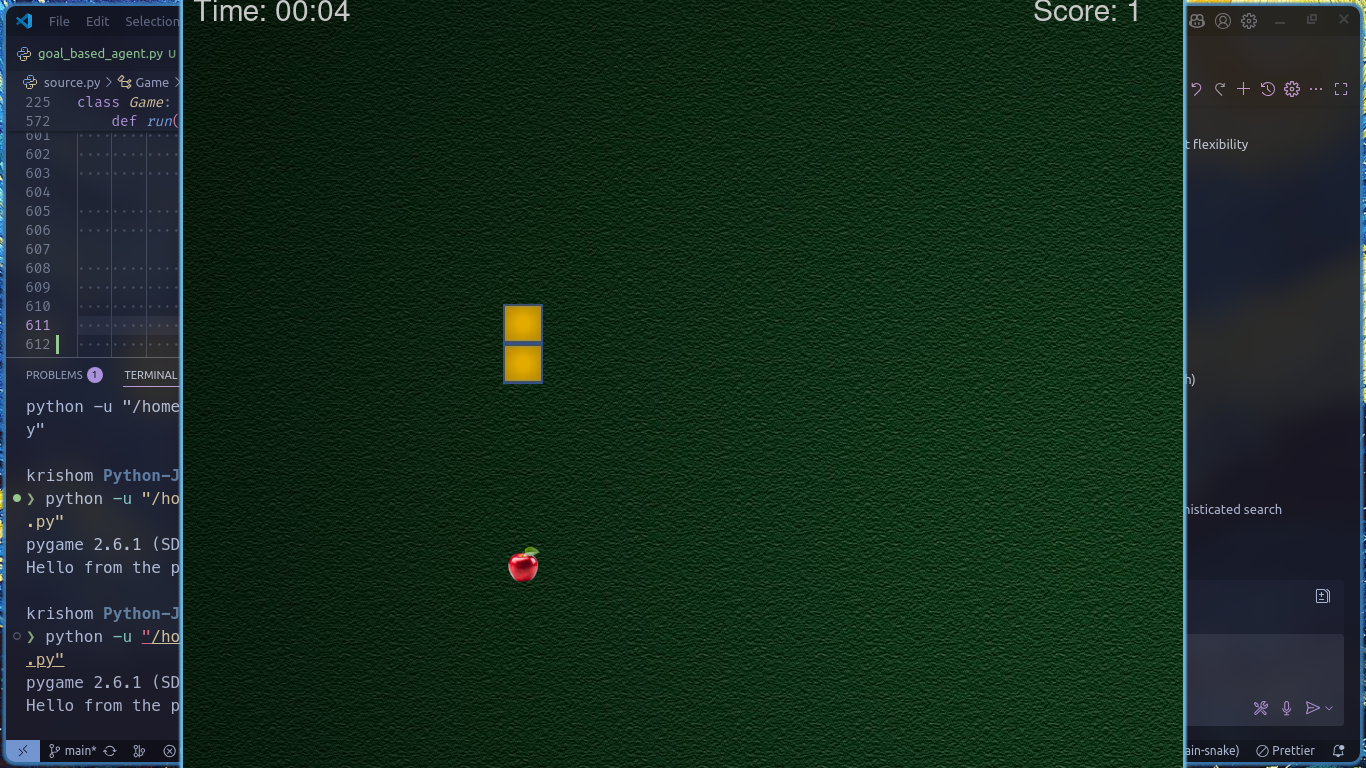
\includegraphics[width=\textwidth]{ss/simple_play.png}
        \caption{Gameplay}
    \end{subfigure}
    \hfill
    \begin{subfigure}{0.45\textwidth}
        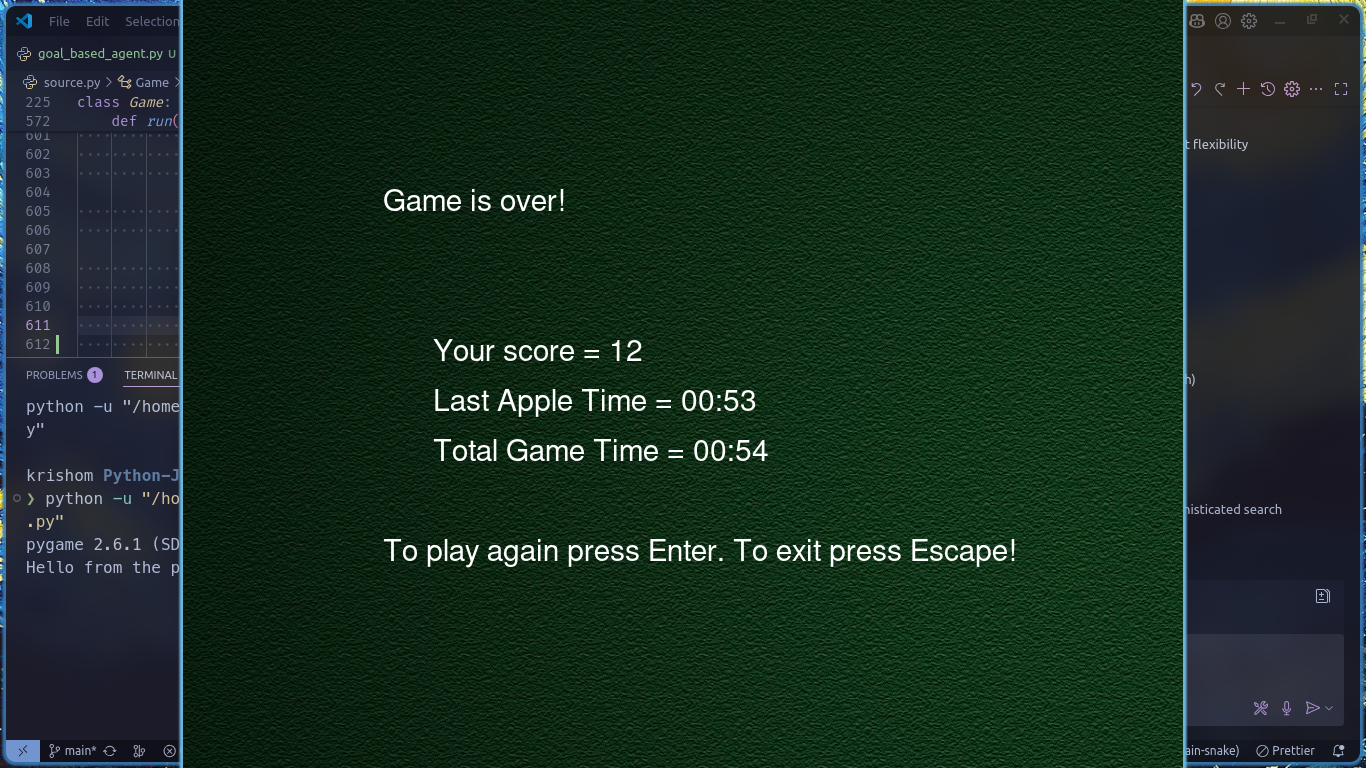
\includegraphics[width=\textwidth]{ss/simple_score.png}
        \caption{Score}
    \end{subfigure}
    \caption{Simple Reflex Agent}
\end{figure}

% ===================== GOAL-BASED AGENT =====================
\section{Goal-Based Agent}
\subsection{Description}
The Goal-Based Agent defines explicit goals (avoid death, reach apple, maximize score, maintain safety) and uses search algorithms (A*, BFS) to plan safe paths to the apple.

\subsection{Code}
\begin{lstlisting}[caption=Goal-Based Agent]
import math
from typing import List, Tuple, Optional
from collections import deque
import heapq
SIZE = 40
class Goals:
    REACH_APPLE = "reach_apple"
    AVOID_DEATH = "avoid_death"
    MAXIMIZE_SCORE = "maximize_score"
    MAINTAIN_SAFETY = "maintain_safety"
def goal_based_agent(game):
    """
    A true goal-based agent that:
    1. Defines explicit goals
    2. Plans sequences of actions using search algorithms
    3. Considers future states beyond immediate moves
    4. Uses A* pathfinding to achieve goals
    """
    # Get current state
    head_x, head_y = game.snake.x[0], game.snake.y[0]
    apple_x, apple_y = game.apple.x, game.apple.y

    # Goal Priority System
    current_goals = determine_active_goals(game)

    # Goal 1: PRIMARY - Find safe path to apple (REACH_APPLE + AVOID_DEATH)
    if Goals.REACH_APPLE in current_goals:
        path_to_apple = a_star_search(game, (head_x, head_y), (apple_x, apple_y))

        if path_to_apple and len(path_to_apple) > 1:
            # Verify the path is still safe after planning
            if is_path_safe(game, path_to_apple):
                next_move = get_direction_from_positions(
                    head_x, head_y, path_to_apple[1][0], path_to_apple[1][1]
                )
                execute_move(game, next_move)
                return

    # Goal 2: SAFETY - Maintain safe space when no direct path to apple
    if Goals.MAINTAIN_SAFETY in current_goals:
        safe_exploration_move = find_safe_exploration_move(game)
        if safe_exploration_move:
            execute_move(game, safe_exploration_move)
            return

    # Goal 3: MAXIMIZE_SCORE - Use BFS to find any reachable apple path
    if Goals.MAXIMIZE_SCORE in current_goals:
        bfs_path = bfs_search(game, (head_x, head_y), (apple_x, apple_y))
        if bfs_path and len(bfs_path) > 1:
            next_move = get_direction_from_positions(
                head_x, head_y, bfs_path[1][0], bfs_path[1][1]
            )
            execute_move(game, next_move)
            return

    # Goal 4: AVOID_DEATH - Emergency survival mode
    emergency_move(game)
\end{lstlisting}

\subsection{Screenshots}
\begin{figure}[H]
    \centering
    \begin{subfigure}{0.45\textwidth}
        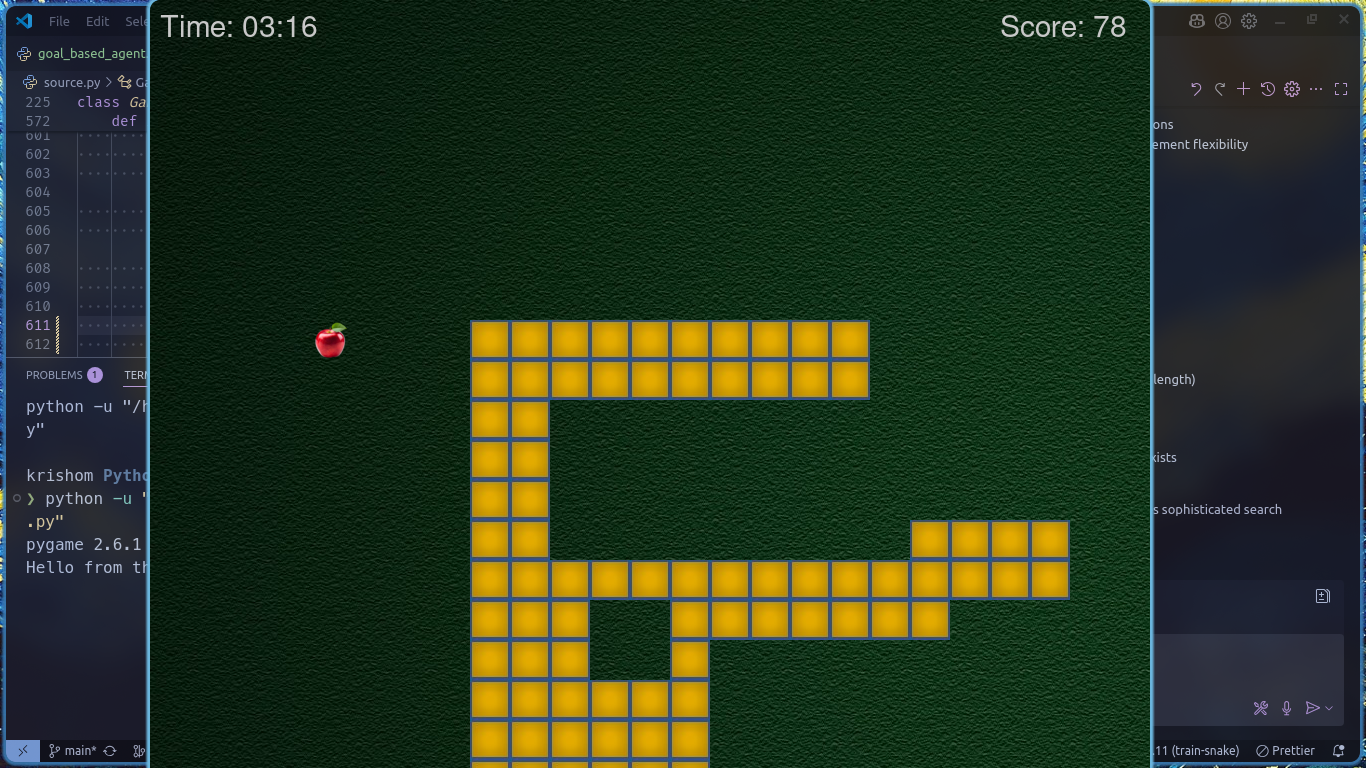
\includegraphics[width=\textwidth]{ss/goal_based_play.png}
        \caption{Gameplay}
    \end{subfigure}
    \hfill
    \begin{subfigure}{0.45\textwidth}
        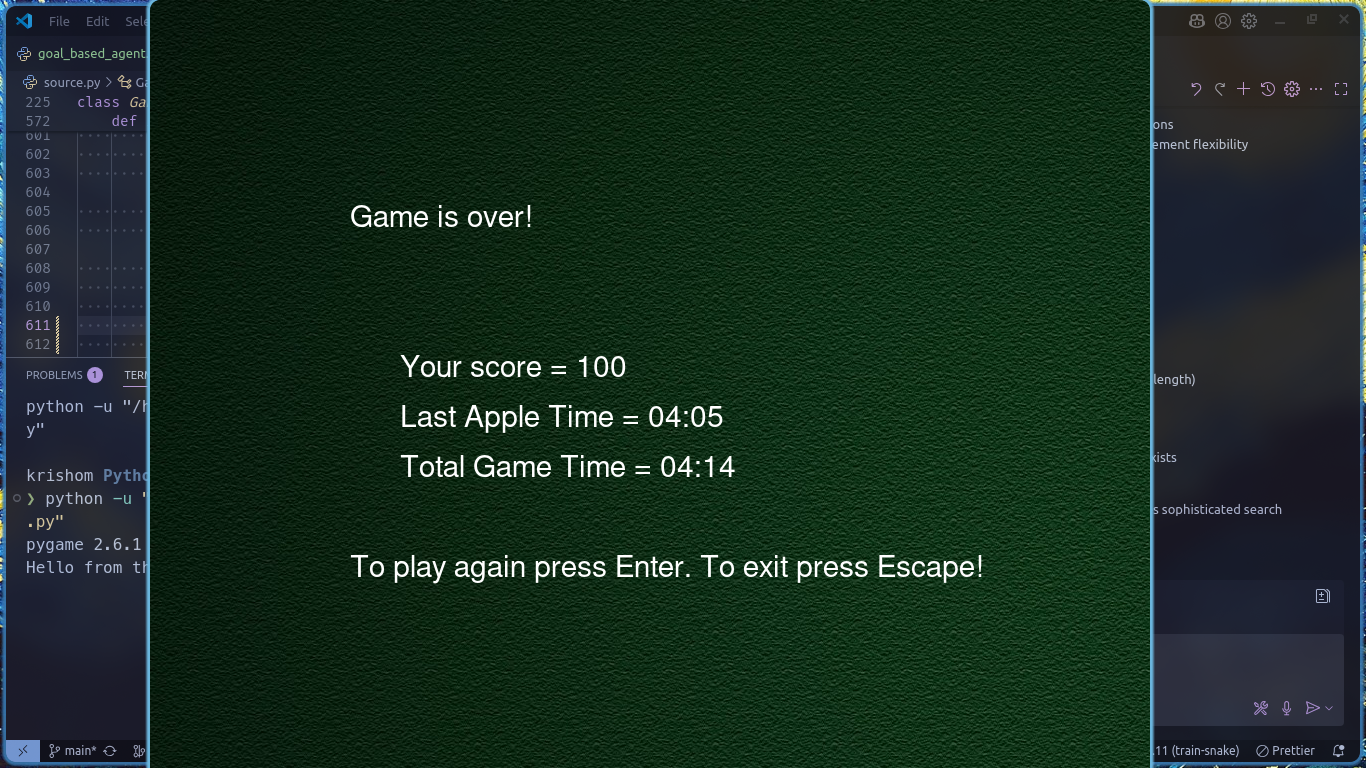
\includegraphics[width=\textwidth]{ss/goal_based_result.png}
        \caption{Score}
    \end{subfigure}
    \caption{Goal-Based Agent}
\end{figure}

% ===================== UTILITY-BASED AGENT =====================
\section{Utility-Based Agent}
\subsection{Description}
The Utility-Based Agent evaluates each possible action using a utility function that combines food attraction, safety, space, and efficiency. It chooses the action with the highest utility score.

\subsection{Code}
\begin{lstlisting}[caption=Utility-Based Agent]
def utility_based_agent(game):
    """
    Utility-Based Agent that evaluates actions based on a utility function:
    1. Considers multiple factors: food attraction, safety, space, efficiency
    2. Computes a utility score for each possible actionw
    3. Selects the action with the highest utility score
    """
    head_x, head_y = game.snake.x[0], game.snake.y[0]
    apple_x, apple_y = game.apple.x, game.apple.y

    def compute_utility(action: str) -> float:
        """Compute utility score for a given action"""
        next_x, next_y = game._get_potential_head(action)

        # Basic safety check
        if game._is_potential_move_colliding(next_x, next_y):
            return float("-inf")  # Avoid dangerous moves

        utility = 0.0

        # Factor 1: Food attraction (distance to apple)
        distance_to_apple = abs(apple_x - next_x) + abs(apple_y - next_y)
        utility -= distance_to_apple  # Closer is better

        # Factor 2: Safety (avoid danger zones)
        if (next_x, next_y) in danger_zones:
            utility += 100  # Penalize moves into danger zones

        # Factor 3: Space (prefer moves with more free space)
        free_space = count_free_space_around(game, next_x, next_y)
        utility += free_space  # More free space is better

        # Factor 4: Efficiency (penalize unnecessary moves)
        if action in ["left", "right"]:
            utility -= 1  # Penalize horizontal moves
        elif action in ["up", "down"]:
            utility -= 1  # Penalize vertical moves

        return utility

    # Evaluate all possible actions and select the best one
    possible_actions = ["left", "right", "up", "down"]
    best_action = max(possible_actions, key=compute_utility)

    # Execute the best action
    if best_action == "left":
        game.snake.move_left()
    elif best_action == "right":
        game.snake.move_right()
    elif best_action == "up":
        game.snake.move_up()
    elif best_action == "down":
        game.snake.move_down()
\end{lstlisting}

\subsection{Screenshots}
\begin{figure}[H]
    \centering
    \begin{subfigure}{0.45\textwidth}
        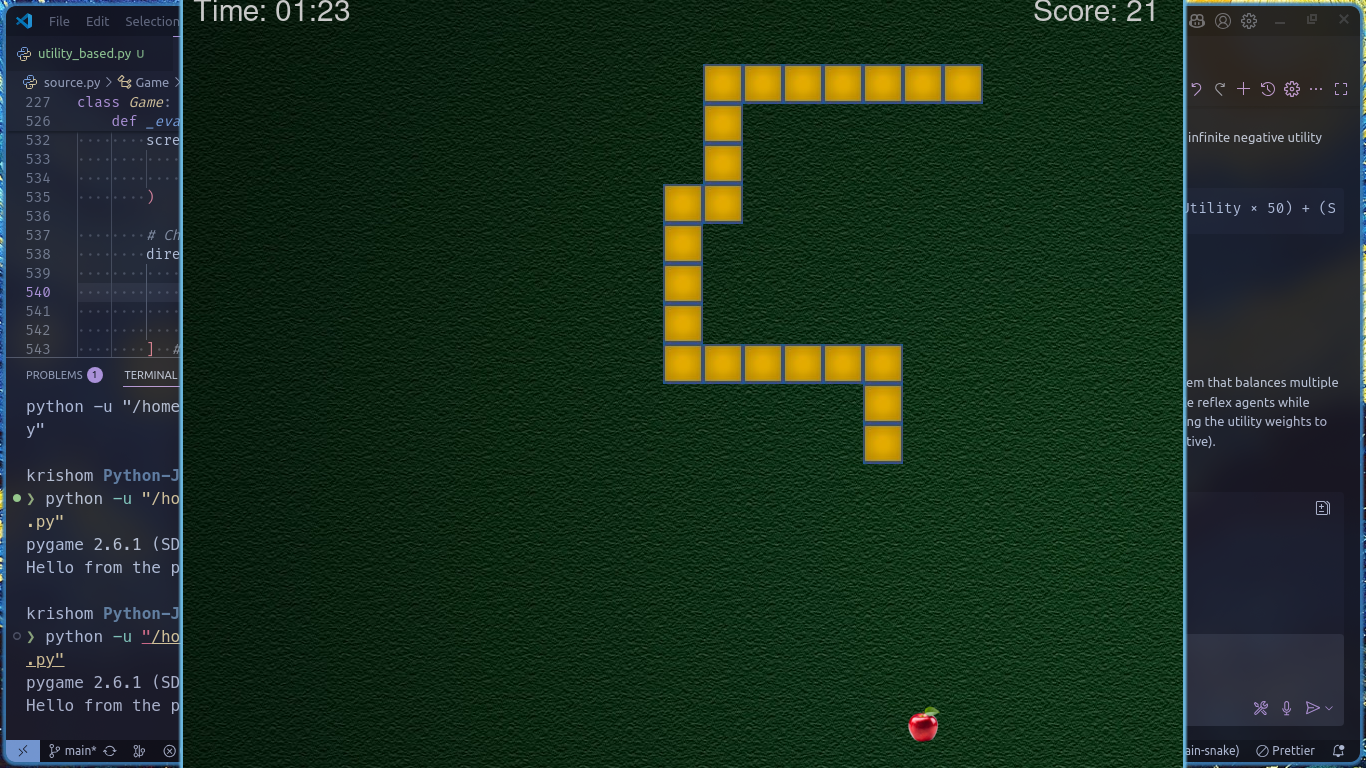
\includegraphics[width=\textwidth]{ss/utility_based_play.png}
        \caption{Gameplay}
    \end{subfigure}
    \hfill
    \begin{subfigure}{0.45\textwidth}
        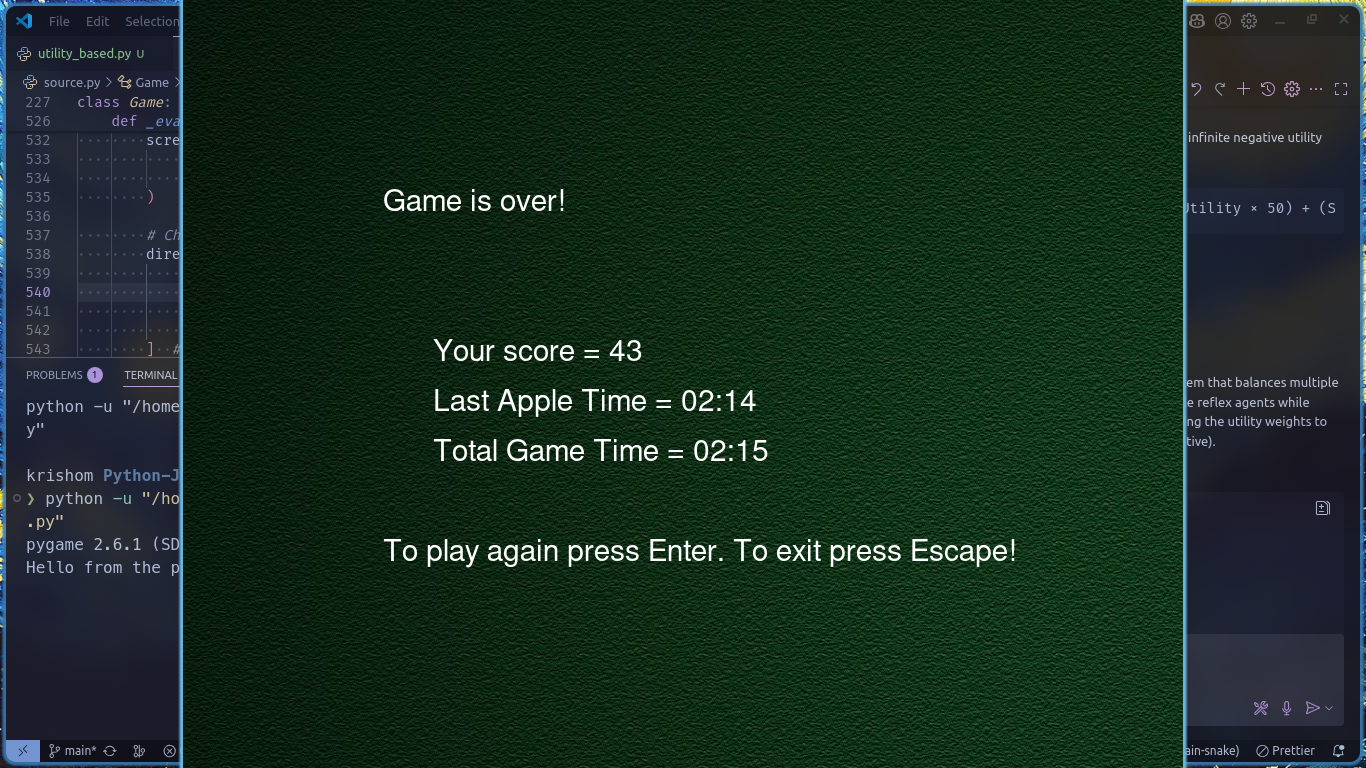
\includegraphics[width=\textwidth]{ss/utility_based_score.png}
        \caption{Score}
    \end{subfigure}
    \caption{Utility-Based Agent}
\end{figure}

% ===================== MODEL-BASED AGENT =====================
\section{Model-Based Agent}
\subsection{Description}
The Model-Based Agent maintains an internal world model, learns from experience, and adapts its strategy over time. It remembers dangerous positions, successful moves, and uses this knowledge to make safer, more effective decisions.

\subsection{Code}
\begin{lstlisting}[caption=Model-Based Agent]
def model_based_agent(game):
    """
    Model-Based Agent with persistent world model and learning capabilities
    
    Key Requirements Met:
    1. Internal State Storage
    2. World Model (game mechanics understanding)  
    3. Learning from Experience
    4. Model-based Decision Making
    """
    global _world_model

    # REQUIREMENT 1: Internal State Storage
    if _world_model is None:
        _world_model = {
            "apple_positions": [],      # Track apple movement pattern
            "danger_zones": set(),      # Remember dangerous positions
            "safe_moves": {},          # Remember successful moves
            "collision_near_misses": [], # Learn from close calls
            "movement_history": [],     # Track movement patterns
            "step_count": 0,           # Track game progression
        }

    world_model = _world_model
    world_model["step_count"] += 1

    # REQUIREMENT 2: World Model - Update understanding of game mechanics
    update_world_model(world_model, current_state, game)

    # REQUIREMENT 3: Learning from Experience
    learn_from_experience(world_model, current_state, game)

    # REQUIREMENT 4: Model-based Decision Making
    action = make_model_based_decision(world_model, current_state, game)
\end{lstlisting}

\subsection{Screenshots}
\begin{figure}[H]
    \centering
    \begin{subfigure}{0.45\textwidth}
        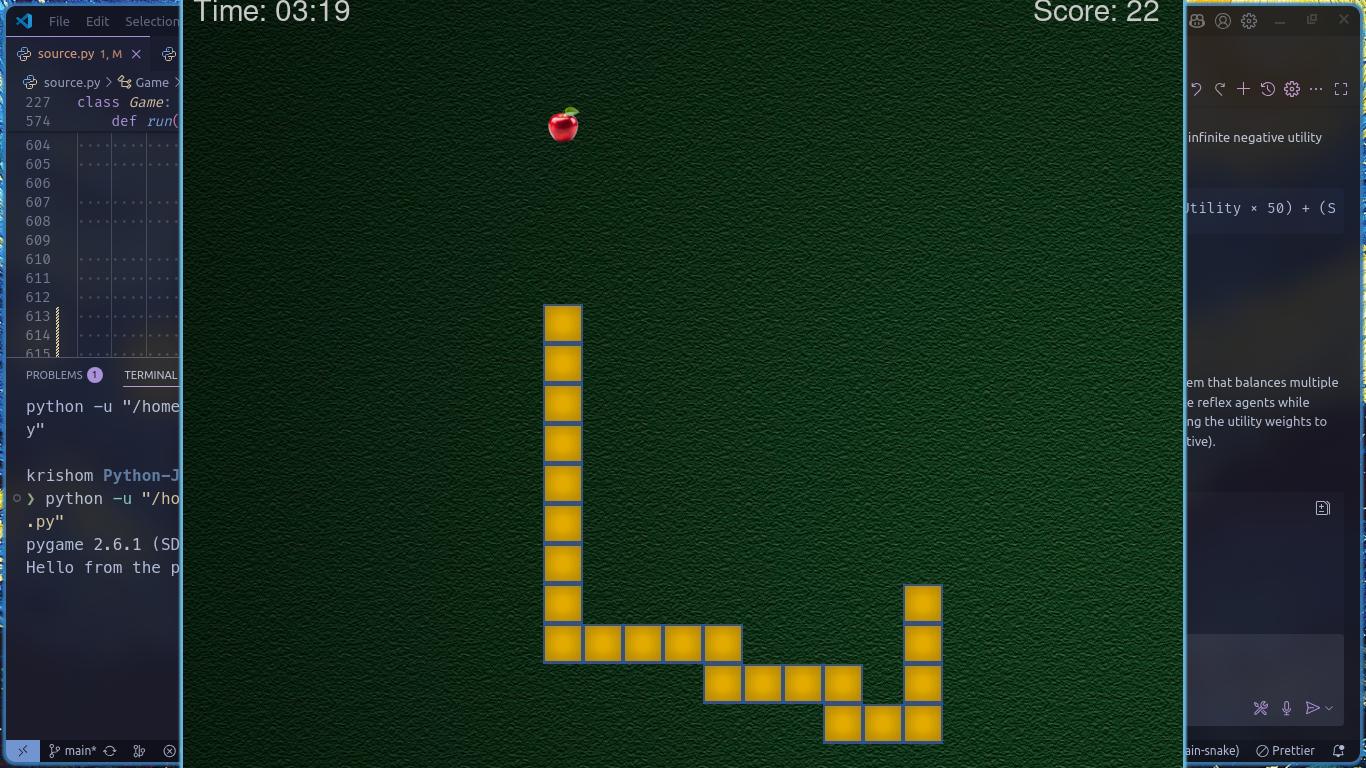
\includegraphics[width=\textwidth]{ss/model_based_play.png}
        \caption{Gameplay}
    \end{subfigure}
    \hfill
    \begin{subfigure}{0.45\textwidth}
        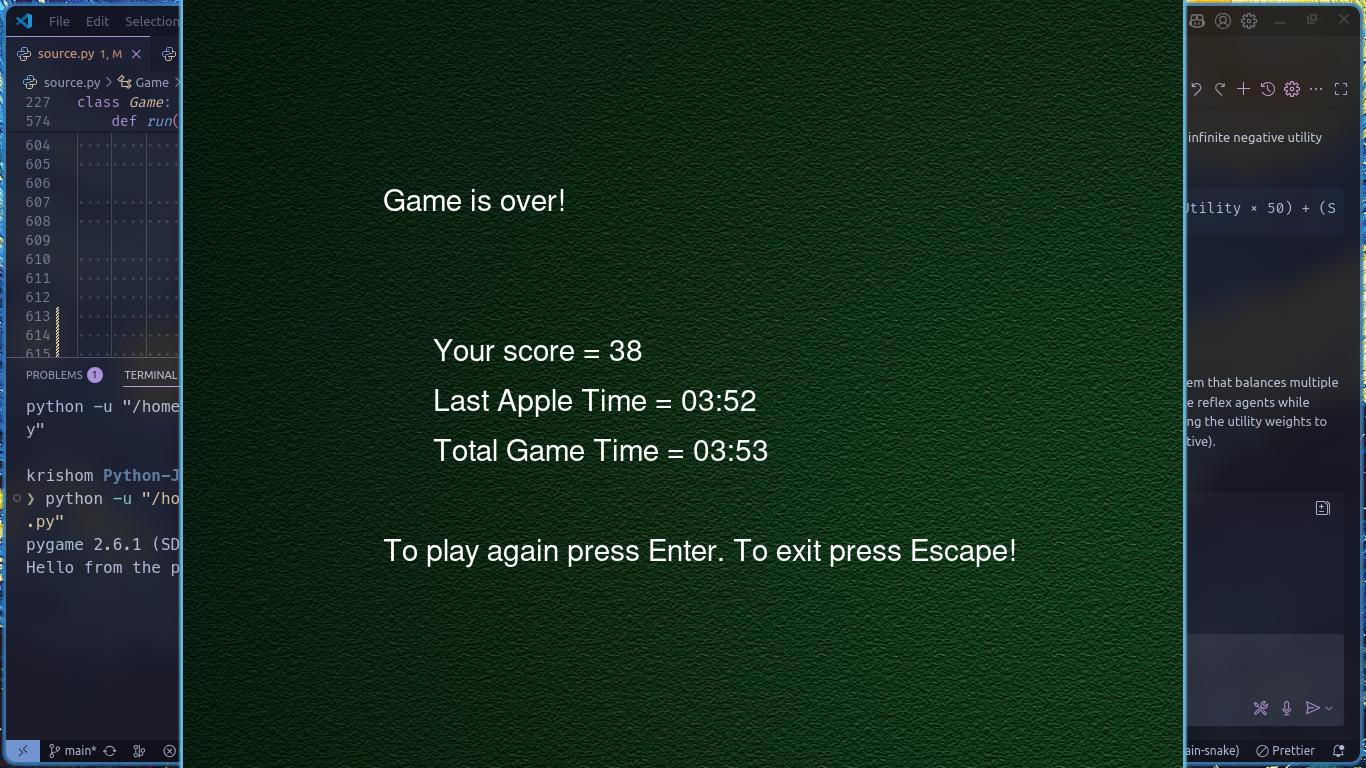
\includegraphics[width=\textwidth]{ss/model_based_score.png}
        \caption{Score}
    \end{subfigure}
    \caption{Model-Based Agent}
\end{figure}

% ===================== Q-LEARNING AGENT =====================
\section{Q-Learning Agent (Reinforcement Learning)}
\subsection{Description}
The Q-Learning Agent uses reinforcement learning to discover optimal strategies through trial and error. It maintains a Q-table that stores quality scores for state-action pairs, using simplified state representation to overcome the curse of dimensionality. The agent learns from rewards (+50 for apples, -100 for collisions, -1 per move) and gradually improves its performance over time.

\subsection{Code}
\begin{lstlisting}[caption=Q-Learning Agent]
def learning_model(game):
    """
    Q-Learning Agent that learns optimal strategies through experience:
    1. Uses simplified state representation (apple direction, distance, dangers)
    2. Maintains Q-table with quality scores for state-action pairs
    3. Employs epsilon-greedy exploration/exploitation strategy
    4. Learns from rewards and updates Q-values using Bellman equation
    5. Saves/loads knowledge for persistent learning across sessions
    """
    global last_state, last_action, last_score, game_count
    
    # Load Q-table on first run
    if game_count == 0:
        load_q_table()
        game_count += 1
    
    # Get simplified state representation
    current_state = get_simple_state(game)
    current_score = game.snake.length - 1
    
    # Get valid actions (avoid U-turns and collisions)
    current_direction = game.snake.direction
    all_actions = ["left", "right", "up", "down"]
    opposite = {"left": "right", "right": "left", "up": "down", "down": "up"}
    
    valid_actions = []
    for action in all_actions:
        if action != opposite.get(current_direction):
            next_x, next_y = game._get_potential_head(action)
            if not game._is_potential_move_colliding(next_x, next_y):
                valid_actions.append(action)
    
    # Update Q-table with previous experience
    if last_state is not None and last_action is not None:
        reward = get_reward(game, last_score, current_score, False)
        update_q_table(last_state, last_action, reward, current_state, valid_actions)
    
    # Choose action using epsilon-greedy strategy
    if valid_actions:
        action = choose_action(current_state, valid_actions)
        
        # Execute chosen action
        if action == "left":
            game.snake.move_left()
        elif action == "right":
            game.snake.move_right()
        elif action == "up":
            game.snake.move_up()
        elif action == "down":
            game.snake.move_down()
        
        # Store state for next iteration
        last_state = current_state
        last_action = action
        last_score = current_score

def get_simple_state(game):
    """Create simplified state representation to avoid curse of dimensionality"""
    head_x, head_y = game.snake.x[0], game.snake.y[0]
    apple_x, apple_y = game.apple.x, game.apple.y
    
    # Relative apple position
    horizontal = "right" if apple_x > head_x else "left" if apple_x < head_x else "same"
    vertical = "down" if apple_y > head_y else "up" if apple_y < head_y else "same"
    
    # Distance bucket
    distance = abs(apple_x - head_x) + abs(apple_y - head_y)
    dist_bucket = ("very_close" if distance <= 40 else "close" if distance <= 120 
                   else "medium" if distance <= 240 else "far")
    
    # Danger detection for each direction
    dangers = {}
    for direction in ["left", "right", "up", "down"]:
        next_x, next_y = game._get_potential_head(direction)
        dangers[direction] = game._is_potential_move_colliding(next_x, next_y)
    
    # Combine into state string
    state = f"{horizontal}_{vertical}_{dist_bucket}_{game.snake.direction}_"
    state += f"L{dangers['left']}_R{dangers['right']}_U{dangers['up']}_D{dangers['down']}"
    return state

def choose_action(state, valid_actions):
    """Epsilon-greedy action selection: 10% exploration, 90% exploitation"""
    if random.random() < 0.1:  # Explore
        return random.choice(valid_actions)
    else:  # Exploit
        best_action = max(valid_actions, key=lambda a: q_table[state][a])
        return best_action
\end{lstlisting}

\subsection{Key Features}
\begin{itemize}
\item \textbf{State Space Reduction}: Uses simplified features (apple direction, distance, collision dangers) instead of full grid representation
\item \textbf{Q-Learning Algorithm}: Implements tabular Q-learning with Bellman equation updates
\item \textbf{Exploration vs Exploitation}: 10\% random exploration, 90\% greedy exploitation using epsilon-greedy strategy
\item \textbf{Reward Engineering}: +50 for eating apples, -100 for collisions, -1 per move to encourage efficiency
\item \textbf{Persistent Learning}: Saves/loads Q-table to JSON file for continuous improvement across sessions
\item \textbf{Learning Parameters}: Learning rate α=0.1, discount factor γ=0.95
\item \textbf{Training Metrics}: Comprehensive tracking of episodes, steps, scores, exploration rate, and Q-table growth
\end{itemize}

\subsection{Training Measurement}
The Q-Learning agent includes comprehensive training metrics to measure learning progress:

\begin{table}[H]
\centering
\caption{Training Metrics and Measurements}
\begin{tabular}{@{}ll@{}}
\toprule
\textbf{Metric} & \textbf{Description} \\
\midrule
Episodes Completed & Number of complete games played (start to collision) \\
Total Steps/Actions & Cumulative moves made across all episodes \\
Best Score Achieved & Highest number of apples eaten in a single episode \\
Average Score Trend & Rolling average performance over last 100 episodes \\
Exploration Rate & Percentage of random actions vs learned actions \\
Q-Table Size & Number of unique state-action pairs learned \\
Episode Length & Average survival time showing learning progress \\
Training Time & Total time spent in learning sessions \\
\bottomrule
\end{tabular}
\end{table}

\textbf{Training Quality Indicators:}
\begin{itemize}
\item \textit{Good Training}: Rising average scores, growing Q-table, longer episodes
\item \textit{Learning Progress}: Decreasing exploration rate, improving best scores
\item \textit{Convergence}: Stabilizing performance after sufficient episodes (100+)
\end{itemize}

\subsection{Screenshots}
\begin{figure}[H]
    \centering
    \begin{subfigure}{0.45\textwidth}
        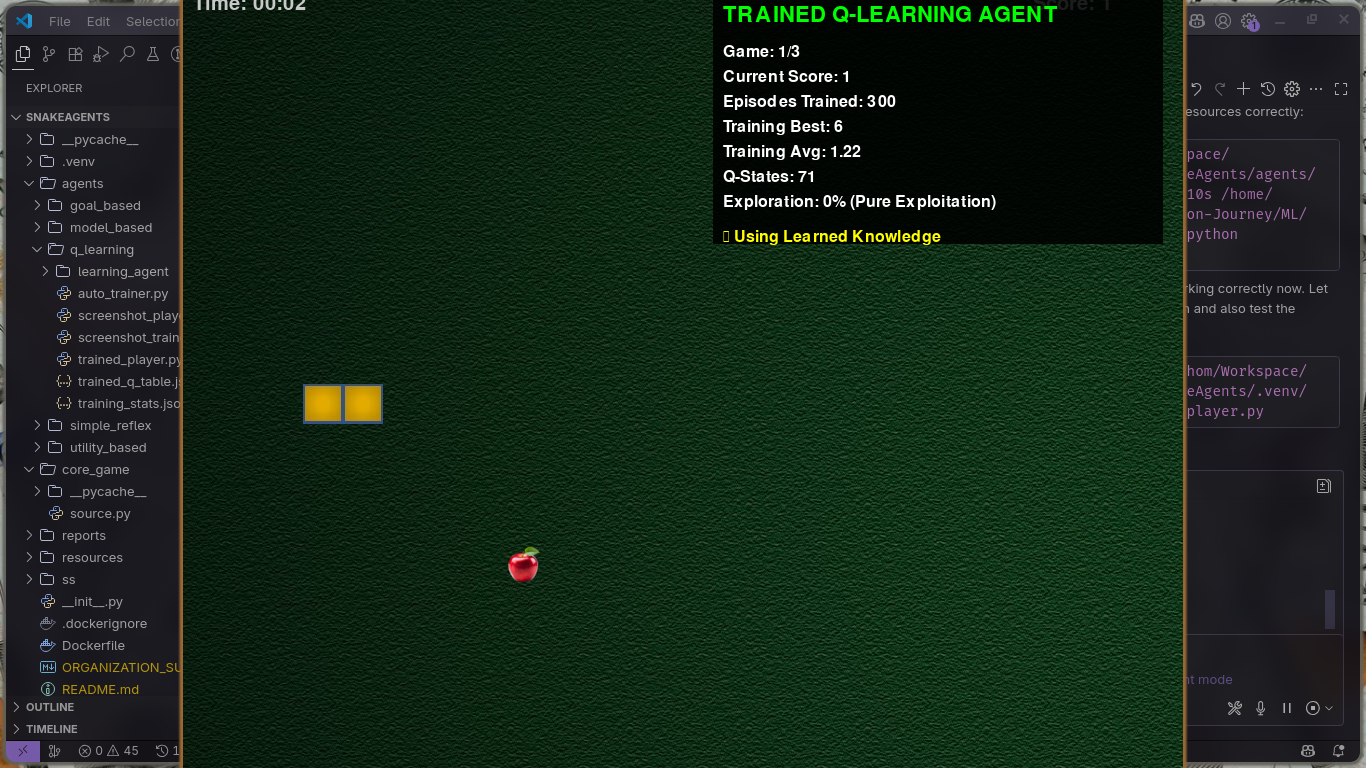
\includegraphics[width=\textwidth]{ss/learning_play.png}
        \caption{Gameplay - Learning in Progress}
    \end{subfigure}
    \hfill
    \begin{subfigure}{0.45\textwidth}
        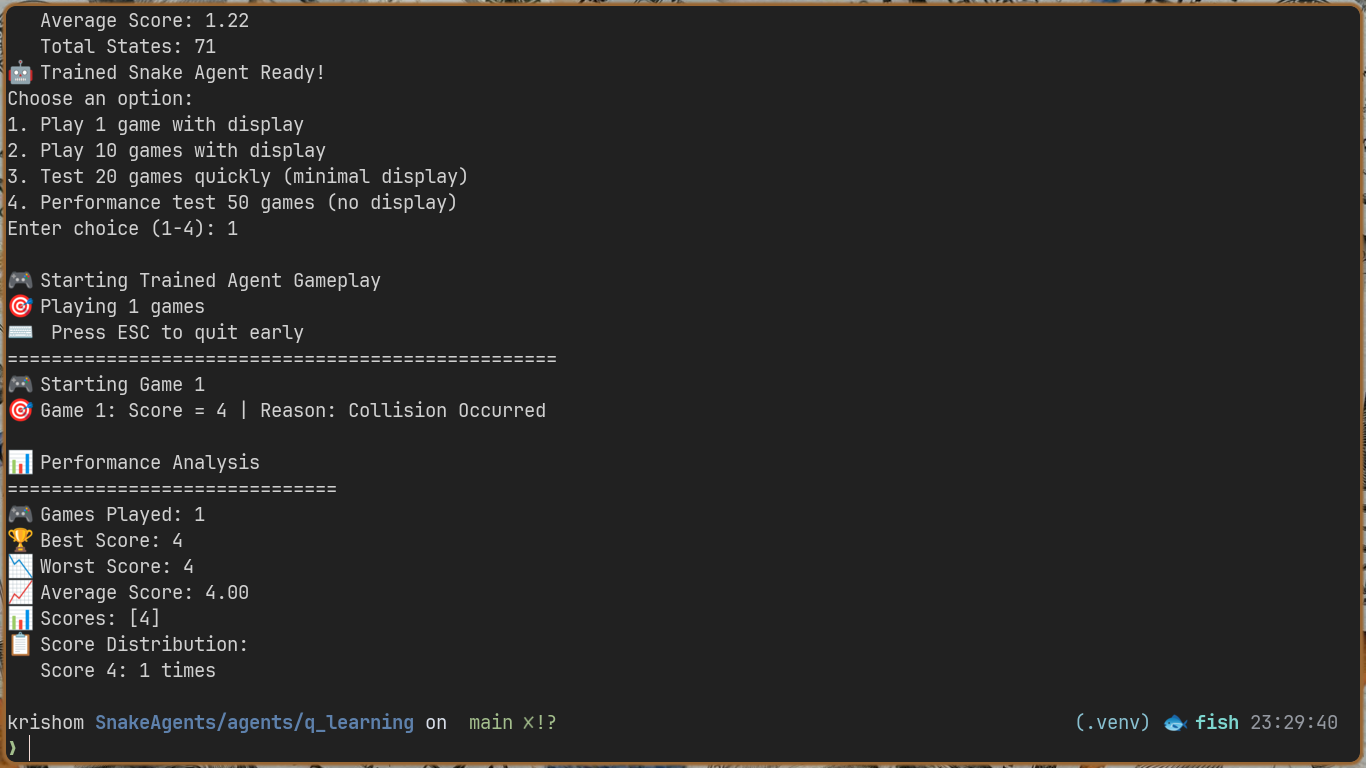
\includegraphics[width=\textwidth]{ss/learning_score.png}
        \caption{Performance Improvement Over Time}
    \end{subfigure}
    \caption{Q-Learning Agent}
\end{figure}

% ===================== COMPARISON =====================
\section{Comparative Summary}
\begin{table}[H]
\centering
\caption{Agent Comparison}
\begin{tabular}{@{}lccccc@{}}
\toprule
\textbf{Characteristic} & \textbf{Simple Reflex} & \textbf{Goal-Based} & \textbf{Utility-Based} & \textbf{Model-Based} & \textbf{Q-Learning} \\
\midrule
Decision Making & Reactive & Proactive & Utility Optimization & Adaptive & Learned Policy \\
Planning Horizon & 1 step & Multi-step & Multi-factor & Learned Experience & Experience-Based \\
Search Algorithm & None & A*, BFS & Utility Function & Model-Based Eval & Q-Learning \\
Learning Capability & None & None & None & Experience-Based & Reinforcement \\
Memory & None & Temporary & None & Persistent & Q-Table \\
State Representation & Current Position & Full State & Current State & World Model & Simplified Features \\
Adaptation & None & None & None & Strategy Learning & Policy Learning \\
Performance & Moderate & Superior & Flexible & Optimal & Improving \\
\bottomrule
\end{tabular}
\end{table}

\section{Conclusion}
This report demonstrates the progression from simple reactive agents to sophisticated learning agents in the Snake game. Each agent type offers unique strengths and trade-offs:

\begin{itemize}
\item \textbf{Simple Reflex Agent}: Basic reactive behavior, suitable for simple environments
\item \textbf{Goal-Based Agent}: Strategic planning with search algorithms for optimal pathfinding
\item \textbf{Utility-Based Agent}: Multi-criteria decision making with flexible preference modeling
\item \textbf{Model-Based Agent}: Adaptive behavior through experience and world model maintenance
\item \textbf{Q-Learning Agent}: Autonomous learning through reinforcement, discovering optimal policies without prior knowledge
\end{itemize}

The Q-Learning agent represents the pinnacle of autonomous intelligence, capable of improving performance through trial and error while requiring no pre-programmed strategies. This progression illustrates the evolution from hand-coded intelligence to machine-learned intelligence, demonstrating the power of reinforcement learning in creating truly adaptive artificial agents.

\end{document}